\documentclass{standalone}
\usepackage{tikz}
\usetikzlibrary{patterns, positioning}

\begin{document}
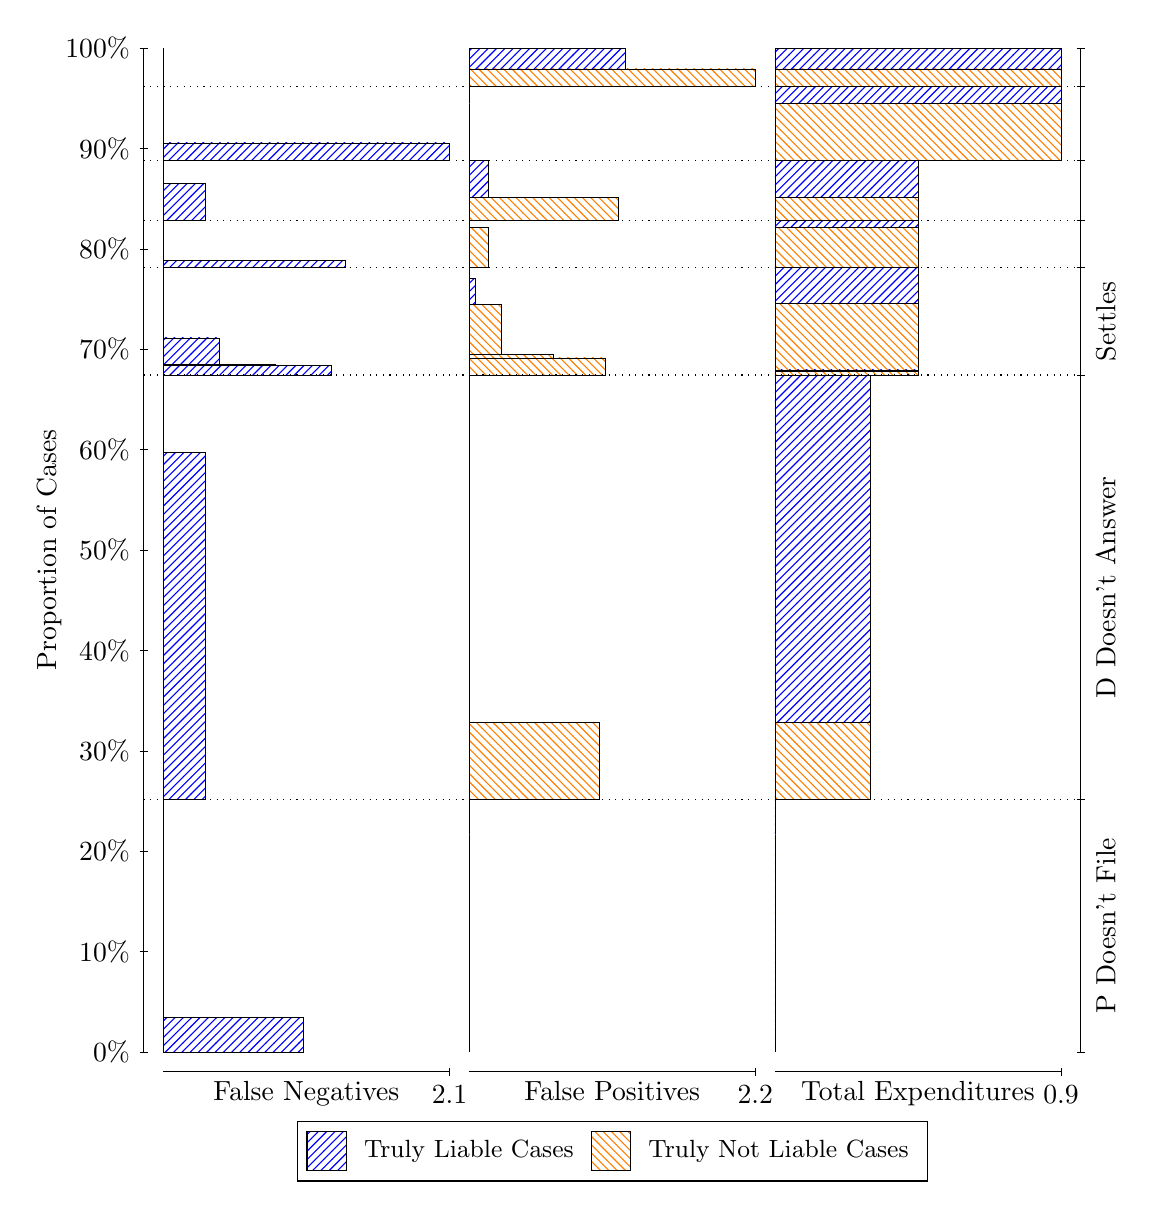
\begin{tikzpicture}
\draw[black, very thin] (1.5,1.75) -- (1.5,14.5);
\node[rotate=90, anchor=center] at (0.3, 8.125) {Proportion of Cases};
\draw[black, very thin] (1.45,1.75) -- (1.55,1.75);
\node[anchor=east] at (1.45, 1.75) {0\%};
\draw[black, very thin] (1.45,3.025) -- (1.55,3.025);
\node[anchor=east] at (1.45, 3.025) {10\%};
\draw[black, very thin] (1.45,4.3) -- (1.55,4.3);
\node[anchor=east] at (1.45, 4.3) {20\%};
\draw[black, very thin] (1.45,5.575) -- (1.55,5.575);
\node[anchor=east] at (1.45, 5.575) {30\%};
\draw[black, very thin] (1.45,6.85) -- (1.55,6.85);
\node[anchor=east] at (1.45, 6.85) {40\%};
\draw[black, very thin] (1.45,8.125) -- (1.55,8.125);
\node[anchor=east] at (1.45, 8.125) {50\%};
\draw[black, very thin] (1.45,9.4) -- (1.55,9.4);
\node[anchor=east] at (1.45, 9.4) {60\%};
\draw[black, very thin] (1.45,10.675) -- (1.55,10.675);
\node[anchor=east] at (1.45, 10.675) {70\%};
\draw[black, very thin] (1.45,11.95) -- (1.55,11.95);
\node[anchor=east] at (1.45, 11.95) {80\%};
\draw[black, very thin] (1.45,13.225) -- (1.55,13.225);
\node[anchor=east] at (1.45, 13.225) {90\%};
\draw[black, very thin] (1.45,14.5) -- (1.55,14.5);
\node[anchor=east] at (1.45, 14.5) {100\%};

\draw[black, very thin] (13.4,1.75) -- (13.4,14.5);
\draw[black, very thin] (13.35,1.75) -- (13.45,1.75);
\node[anchor=west] at (13.35, 1.75) {};
\draw[black, very thin] (13.35,4.954) -- (13.45,4.954);
\node[anchor=west] at (13.35, 4.954) {};
\draw[black, very thin] (13.35,10.347) -- (13.45,10.347);
\node[anchor=west] at (13.35, 10.347) {};
\draw[black, very thin] (13.35,11.714) -- (13.45,11.714);
\node[anchor=west] at (13.35, 11.714) {};
\draw[black, very thin] (13.35,12.313) -- (13.45,12.313);
\node[anchor=west] at (13.35, 12.313) {};
\draw[black, very thin] (13.35,13.072) -- (13.45,13.072);
\node[anchor=west] at (13.35, 13.072) {};
\draw[black, very thin] (13.35,14.016) -- (13.45,14.016);
\node[anchor=west] at (13.35, 14.016) {};
\draw[black, very thin] (13.35,14.5) -- (13.45,14.5);
\node[anchor=west] at (13.35, 14.5) {};

\draw[black, very thin, pattern color=blue, pattern=north east lines] (1.75,1.75) rectangle (3.5224,2.1915);
\draw[black, very thin, pattern color=orange, pattern=north west lines] (1.75,2.1915) rectangle (1.75,4.954);
\draw[black, very thin, pattern color=blue, pattern=north east lines] (1.75,4.954) rectangle (2.2817,9.3676);
\draw[black, very thin, pattern color=orange, pattern=north west lines] (1.75,9.3676) rectangle (1.75,10.347);
\draw[black, very thin, pattern color=blue, pattern=north east lines] (1.75,10.347) rectangle (3.8768,10.466);
\draw[black, very thin, pattern color=blue, pattern=north east lines] (1.75,10.466) rectangle (3.1679,10.487);
\draw[black, very thin, pattern color=blue, pattern=north east lines] (1.75,10.487) rectangle (2.4589,10.82);
\draw[black, very thin, pattern color=orange, pattern=north west lines] (1.75,10.82) rectangle (1.75,11.714);
\draw[black, very thin, pattern color=blue, pattern=north east lines] (1.75,11.714) rectangle (4.0541,11.803);
\draw[black, very thin, pattern color=orange, pattern=north west lines] (1.75,11.803) rectangle (1.75,12.313);
\draw[black, very thin, pattern color=blue, pattern=north east lines] (1.75,12.313) rectangle (2.2817,12.785);
\draw[black, very thin, pattern color=orange, pattern=north west lines] (1.75,12.785) rectangle (1.75,13.072);
\draw[black, very thin, pattern color=blue, pattern=north east lines] (1.75,13.072) rectangle (5.3833,13.294);
\draw[black, very thin, pattern color=orange, pattern=north west lines] (1.75,13.294) rectangle (1.75,14.016);
\draw[black, very thin, pattern color=orange, pattern=north west lines] (1.75,14.016) rectangle (1.75,14.236);
\draw[black, very thin, pattern color=blue, pattern=north east lines] (1.75,14.236) rectangle (1.75,14.5);
\draw[black, very thin, pattern color=orange, pattern=north west lines] (5.6333,1.75) rectangle (5.6333,4.5125);
\draw[black, very thin, pattern color=blue, pattern=north east lines] (5.6333,4.5125) rectangle (5.6333,4.954);
\draw[black, very thin, pattern color=orange, pattern=north west lines] (5.6333,4.954) rectangle (7.2848,5.933);
\draw[black, very thin, pattern color=blue, pattern=north east lines] (5.6333,5.933) rectangle (5.6333,10.347);
\draw[black, very thin, pattern color=orange, pattern=north west lines] (5.6333,10.347) rectangle (7.3674,10.564);
\draw[black, very thin, pattern color=orange, pattern=north west lines] (5.6333,10.564) rectangle (6.7068,10.61);
\draw[black, very thin, pattern color=orange, pattern=north west lines] (5.6333,10.61) rectangle (6.0462,11.24);
\draw[black, very thin, pattern color=blue, pattern=north east lines] (5.6333,11.24) rectangle (5.7159,11.574);
\draw[black, very thin, pattern color=blue, pattern=north east lines] (5.6333,11.574) rectangle (5.6333,11.714);
\draw[black, very thin, pattern color=orange, pattern=north west lines] (5.6333,11.714) rectangle (5.8811,12.224);
\draw[black, very thin, pattern color=blue, pattern=north east lines] (5.6333,12.224) rectangle (5.6333,12.313);
\draw[black, very thin, pattern color=orange, pattern=north west lines] (5.6333,12.313) rectangle (7.5326,12.601);
\draw[black, very thin, pattern color=blue, pattern=north east lines] (5.6333,12.601) rectangle (5.8811,13.072);
\draw[black, very thin, pattern color=orange, pattern=north west lines] (5.6333,13.072) rectangle (5.6333,13.794);
\draw[black, very thin, pattern color=blue, pattern=north east lines] (5.6333,13.794) rectangle (5.6333,14.016);
\draw[black, very thin, pattern color=orange, pattern=north west lines] (5.6333,14.016) rectangle (9.2667,14.236);
\draw[black, very thin, pattern color=blue, pattern=north east lines] (5.6333,14.236) rectangle (7.6152,14.5);
\draw[black, very thin, pattern color=orange, pattern=north west lines] (9.5167,1.75) rectangle (9.5167,4.5125);
\draw[black, very thin, pattern color=blue, pattern=north east lines] (9.5167,4.5125) rectangle (9.5167,4.954);
\draw[black, very thin, pattern color=orange, pattern=north west lines] (9.5167,4.954) rectangle (10.728,5.933);
\draw[black, very thin, pattern color=blue, pattern=north east lines] (9.5167,5.933) rectangle (10.728,10.347);
\draw[black, very thin, pattern color=orange, pattern=north west lines] (9.5167,10.347) rectangle (11.333,10.392);
\draw[black, very thin, pattern color=blue, pattern=north east lines] (9.5167,10.392) rectangle (11.333,10.413);
\draw[black, very thin, pattern color=orange, pattern=north west lines] (9.5167,10.413) rectangle (11.333,11.261);
\draw[black, very thin, pattern color=blue, pattern=north east lines] (9.5167,11.261) rectangle (11.333,11.714);
\draw[black, very thin, pattern color=orange, pattern=north west lines] (9.5167,11.714) rectangle (11.333,12.224);
\draw[black, very thin, pattern color=blue, pattern=north east lines] (9.5167,12.224) rectangle (11.333,12.313);
\draw[black, very thin, pattern color=orange, pattern=north west lines] (9.5167,12.313) rectangle (11.333,12.601);
\draw[black, very thin, pattern color=blue, pattern=north east lines] (9.5167,12.601) rectangle (11.333,13.072);
\draw[black, very thin, pattern color=orange, pattern=north west lines] (9.5167,13.072) rectangle (13.15,13.794);
\draw[black, very thin, pattern color=blue, pattern=north east lines] (9.5167,13.794) rectangle (13.15,14.016);
\draw[black, very thin, pattern color=orange, pattern=north west lines] (9.5167,14.016) rectangle (13.15,14.236);
\draw[black, very thin, pattern color=blue, pattern=north east lines] (9.5167,14.236) rectangle (13.15,14.5);
\draw[black, dotted] (1.5,4.954) -- (13.4,4.954);
\draw[black, dotted] (1.5,10.347) -- (13.4,10.347);
\draw[black, dotted] (1.5,11.714) -- (13.4,11.714);
\draw[black, dotted] (1.5,12.313) -- (13.4,12.313);
\draw[black, dotted] (1.5,13.072) -- (13.4,13.072);
\draw[black, dotted] (1.5,14.016) -- (13.4,14.016);
\draw[black, very thin] (1.75,1.5) -- (5.3833,1.5);
\node[anchor=north] at (3.5667, 1.5) {False Negatives};
\draw[black, very thin] (5.3833,1.45) -- (5.3833,1.55);
\node[anchor=north] at (5.3833, 1.45) {2.1};

\draw[black, very thin] (5.6333,1.5) -- (9.2667,1.5);
\node[anchor=north] at (7.45, 1.5) {False Positives};
\draw[black, very thin] (9.2667,1.45) -- (9.2667,1.55);
\node[anchor=north] at (9.2667, 1.45) {2.2};

\draw[black, very thin] (9.5167,1.5) -- (13.15,1.5);
\node[anchor=north] at (11.333, 1.5) {Total Expenditures};
\draw[black, very thin] (13.15,1.45) -- (13.15,1.55);
\node[anchor=north] at (13.15, 1.45) {0.9};

\node[black, centered, rotate=90] at (13.72, 3.352) {P Doesn't File};
\node[black, centered, rotate=90] at (13.72, 7.6503) {D Doesn't Answer};
\node[black, centered, rotate=90] at (13.72, 11.03) {Settles};





\draw (7.449999999999999,1.5) node[draw=none] (baseCoordinate) {};
\begin{scope}[align=center]
        \matrix[scale=0.5, draw=black, below=0.5cm of baseCoordinate, nodes={draw}, column sep=0.1cm]{
            \node[rectangle, draw, minimum width=0.5cm, minimum height=0.5cm, pattern=north east lines, pattern color=blue] {}; &
            \node[draw=none, font=\small] (B) {Truly Liable Cases}; &
            \node[rectangle, draw, minimum width=0.5cm, minimum height=0.5cm, pattern=north west lines, pattern color=orange] {}; &
            \node[draw=none, font=\small] (B) {Truly Not Liable Cases}; \\
            };
\end{scope}

\end{tikzpicture}
\end{document}